\newcommand{\lecturetitle}[1]{
  \title{01204211 Discrete Mathematics \\ #1}
  \author{Jittat Fakcharoenphol}
  \frame{\titlepage}
}
\newcommand{\Mod}{\,\bmod\,}


\newcommand\sbullet[1][.5]{\mathbin{\vcenter{\hbox{\scalebox{#1}{$\bullet$}}}}}

\lecturetitle{Lecture 10a: Nondeterministic automata\footnote{Based on lecture notes of {\em Models of Computation} course by Jeff Erickson.}} 
\renewcommand{\epsilon}{\varepsilon}

\newcommand{\czero}{{\mathtt 0}}
\newcommand{\cone}{{\mathtt 1}}

\begin{frame}
  \frametitle{Review: DFA (Formal definitions)}

  A {\color{red}\bf finite-state machine} or a {\color{red}\bf
    deterministic finite-state automaton} (DFA) has five components:

  \begin{itemize}
  \item the input alphabet $\Sigma$,
  \item a finite set of states $Q$,
  \item a transition function $\delta$ $:Q\times\Sigma \longrightarrow Q$
  \item a start state $s\in Q$, and
  \item a subset $A\subseteq Q$ of accepting states.
  \end{itemize}
  
\end{frame}

\begin{frame}
  \frametitle{Review: Acceptance}

  {\bf One step move}: from state $q$ with input symbol $a$, the
  machine changes its state to $\delta(q,a)$.

  {\bf Extension:} from state $q$ with input string $w$, the machine
  changes its state to $\delta^*(q,w)$ defined as

  \begin{block}{}
  \[
  \delta^*(q,w) = \left\{
  \begin{array}{ll}
    q & \mbox{if $w=\epsilon$,} \\
    \delta^*(\delta(q,a),x) & \mbox{if $w=ax$.}
  \end{array}
  \right.
  \]
  \end{block}
  
  The signature of $\delta^*$ is $Q\times\Sigma^* \longrightarrow Q$.

  \begin{block}{accepting $w$}   
    For a finite-state machine with starting state $s$ and accepting
    states $A$, it accepts string $w$ iff
    
    \[
    \delta^*(s,w)\in A.
    \]
  \end{block}
\end{frame}

\begin{frame}
  \frametitle{Language of a DFA}

  \begin{block}{$L(M)$}
    For a DFA $M$, let $L(M)$ be the set of all strings that $M$
    accepts.  More formally, for $M=(\Sigma,Q,\delta,s,A)$,
    \[
    L(M)=\{w\in\Sigma^* \;|\; \delta^*(s,w)\in A\}.
    \]
    We refer to $L(M)$ as the language of $M$.
  \end{block}

  \begin{block}{Acceptance}
    We also says $M$ {\color{red}\bf accepts} $L(M)$.
  \end{block}
  
\end{frame}

\frame{

  \frametitle{New example 1}

  \centering{
    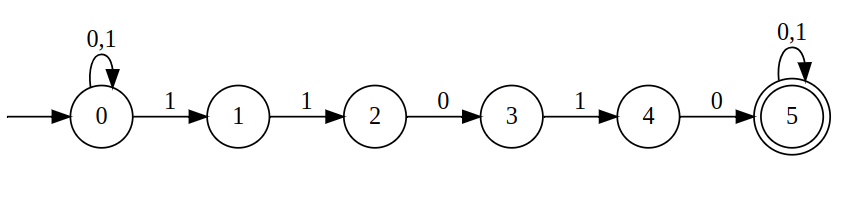
\includegraphics[width=4.5in]{images/gv/mc04-nfa-ex1.png}
  }
}

\frame{

  \frametitle{New example 2}

  \centering{
    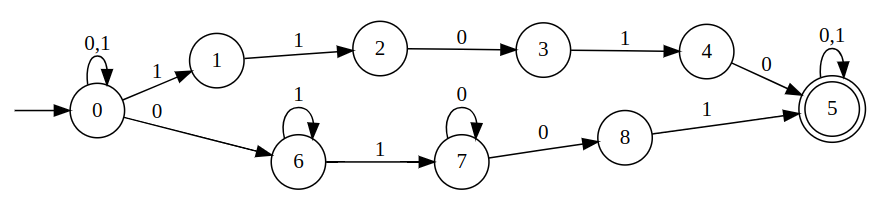
\includegraphics[width=4.5in]{images/gv/mc04-nfa-ex2.png}
  }
}

\frame{

  \frametitle{What's going on here?}
  
}

\frame{
  \frametitle{More relaxed transitions}

  From state $q\in Q$, for input $a$, the machine can ``possibly''
  change its state to many states.

  \pause

  New transition function $\delta :$ \pause $Q\times\Sigma\longrightarrow 2^Q$.

  We refer to this new kind of automaton as a {\color{red}\bf
    nondeterministic finite-state automaton} or {\color{red}\bf NFA}.
}

\begin{frame}
  \frametitle{NFA (Formal definitions)}

  A {\color{red}\bf nondeterministic finite-state automaton} (NFA) has
  five components:

  \begin{itemize}
  \item the input alphabet $\Sigma$, \pause
  \item a finite set of states $Q$, \pause
  \item a transition function $\delta$ \pause $:Q\times\Sigma \longrightarrow 2^Q$ \pause
  \item a start state $s\in Q$, and
  \item a subset $A\subseteq Q$ of accepting states.
  \end{itemize}

  \pause

  Remark: $\delta$ can return the empty set $\emptyset$.

  \pause

  What else do we need to define to ``properly'' talk about NFAs?
\end{frame}

\frame{

  \frametitle{Transition}
  
  {\bf One step move}: from state $q$ with input symbol $a$, the
  machine changes its state to one of $\delta(q,a)$.

  \pause

  Thus, instead of thinking of a machine that maintains {\bf one}
  state, we can think of an NFA as a machine that maintains a {\bf
    set} of states.

  If the current set of states is $C\subseteq Q$ and the input is
  $a\in\Sigma$ what would the new set of states be?

  \pause

  {\bf Extension:} from state $q$ with input string $w$, the machine
  changes its set of states $\delta^*(q,w)$ defined as

  \begin{block}{}
  \[
  \delta^*(q,w) = \left\{
  \begin{array}{ll}
    \{q\} & \mbox{if $w=\epsilon$,} \pause \\
    \\
    {\displaystyle \bigcup_{r\in\delta(q,a)} \delta^*(r,x)} & \mbox{if $w=ax$.}
  \end{array}
  \right.
  \]
  \end{block}
  
  The signature of $\delta^*$ is $Q\times\Sigma^* \longrightarrow 2^Q$.

}

\frame{

  \frametitle{Acceptance}
  
  \begin{block}{accepting $w$}   
    For a nondeterministic finite-state machine with starting state
    $s$ and accepting states $A$, it accepts string $w$ iff
    
    \[
    \delta^*(s,w)\cap A\neq \emptyset.
    \]
  \end{block}
}

\frame{

  \frametitle{Interpretation}

  \pause
  
  \begin{itemize}
  \item
    Clairvoyance.
    \pause

  \item
    Parallel threads.
    \pause

  \item
    Proofs/oracles.

  \end{itemize}

  \vspace{2in}
}

\frame{
  \frametitle{$\epsilon$-transition}

  \pause

  An NFA accepts string $w$ iff there is a sequence of transitions
  \[
  s \stackrel{a_1}{\longrightarrow} q_1
  \stackrel{a_2}{\longrightarrow} q_2
  \stackrel{a_3}{\longrightarrow} q_3
  \stackrel{a_4}{\longrightarrow} 
  \cdots
  \stackrel{a_{k-1}}{\longrightarrow} q_{k-1}
  \stackrel{a_k}{\longrightarrow} q_k,
  \]
  where $q_k\in A$ and $w=a_1a_2\cdots a_k$ where
  $a_i\in\Sigma\cup\{\epsilon\}$ for $1\leq i\leq k$.

  \pause

  The transition function also changes its domain to
  $Q\times(\Sigma\cup\{\epsilon\})$.

}

\frame{
  \frametitle{$\epsilon$-transition: examples}

}

\frame{
  \frametitle{$\epsilon$-reach}

  The $\epsilon$-reach of state $q\in Q$ (denoted by
  $\epsilon$-reach$(q)$) consists of all states $r$ that satisfy one of
  the following conditions:
  \begin{itemize}
  \item $r=q$, or
  \item $r\in\delta(q',\epsilon)$ for some state $q'$ in the
    $\epsilon$-reach of $q$.
  \end{itemize}

}

\frame{
  \frametitle{Extended transition function: $\delta^*$}

  We define $\delta^*:Q\times\Sigma^*\longrightarrow 2^Q$ as follows:
  \[
  \delta^*(p,w) =
  \left\{
  \begin{array}{ll}
    \mbox{$\epsilon$-reach$(p)$} & \mbox{if $w=\epsilon$} \\
    \\
    {
      \displaystyle
      \bigcup_{r\in\mbox{{\scriptsize $\epsilon$-reach$(p)$}}} \;
      \bigcup_{q\in\delta(r,a)}
      \delta^*(q,x)
    }
    & \mbox{if $w=ax$}.
  \end{array}
  \right.  
  \]
}

\frame{
  \frametitle{Notation abuse}

  We sometimes also write, for subset $S\subseteq Q$,
  \[
  \delta(S,a)=\bigcup_{q\in S}\delta(q,a),
  \]
  \pause
  \[
  \delta^*(S,a)=\bigcup_{q\in S}\delta^*(q,a),
  \]
  \pause
  and
  \[
  \mbox{$\epsilon$-reach$(S)$}=\bigcup_{q\in S}\mbox{$\epsilon$-reach$(q)$}.
  \]

}

\frame{
  \frametitle{Extended transition function: $\delta^*$ (with shorter notation)}

  We define $\delta^*:Q\times\Sigma^*\longrightarrow 2^Q$ as follows:
  \[
  \delta^*(p,w) =
  \left\{
  \begin{array}{ll}
    \mbox{$\epsilon$-reach$(p)$} & \mbox{if $w=\epsilon$} \\
    \\
    \delta^*(\delta(\mbox{$\epsilon$-reach$(p)$},a),x)
    & \mbox{if $w=ax$}.
  \end{array}
  \right.  
  \]
}

\frame{
  \frametitle{Removing $\epsilon$-transitions: idea}

}

\frame{
  \begin{lemma}
    For any NFA $M=(\Sigma,Q,\delta,s,A)$ with $\epsilon$-transitions,
    there is an NFA $M'=(\Sigma,Q',\delta',s',A')$ without
    $\epsilon$-transitions such that $L(M)=L(M')$.
  \end{lemma}

  \begin{proof}
    \vspace{2in}
  \end{proof}
}

\frame{
  \frametitle{Main question}

  \begin{itemize}
  \item We see that $\epsilon$-transitions does not add any ``power''
    to the machine.
  \item Does nondeterminism add any power to NFA (over typical DFA)?
  \end{itemize}
}

\frame{
  \frametitle{Simulating parallel machines}

}

\frame{
  \frametitle{Subset construction: idea}
}

\frame{
  \frametitle{NFA to DFA: subset construction}

  Given an NFA $M=(\Sigma,Q,\delta,s,A)$, we can construct an
  equivalent DFA $M'=(\Sigma,Q',\delta',s',A')$ as follows:

  \begin{itemize}
  \item Let $Q' = 2^Q$, 
  \item $s'=\{s\}$, \pause 
  \item $A'=\{S\subseteq Q \;|\; S\cap A\neq \emptyset\}$, 
  \item and let $\delta':$ $Q'\times\Sigma\longrightarrow Q'$ be such
    that \pause
    \[
    \delta'(q',a) = \bigcup_{p\in q'}\delta(p,a),
    \]
    for all $q'\subseteq Q$ and $a\in\Sigma$.
  \end{itemize}
}

\frame{
  \frametitle{Example}
}

\frame{
  
  \begin{block}{Kleene's Theorem}
    Every language $L$ can be described by a regular expression if and
    only if $L$ is the language accepted by a DFA.
  \end{block}

  \pause

  Steps:
  \begin{itemize}
  \item Every DFA can be transformed into an equivalent NFA.
    \pause (trivial) \pause
  \item Every NFA can be transformed into an equivalent DFA.
    \pause (done) \pause
  \item Every regular expression can be transformed into an equivalent NFA.
    \pause (TODO) \pause
  \item Every NFA can be transformed into an equivalent regular
    expression. {\color{red} (only idea)}
  \end{itemize}
}

\frame{
  \frametitle{Warm-up: union of DFA $\Longrightarrow$ NFA}
    \begin{columns}

    \column{.5\textwidth} {
      \begin{center}
        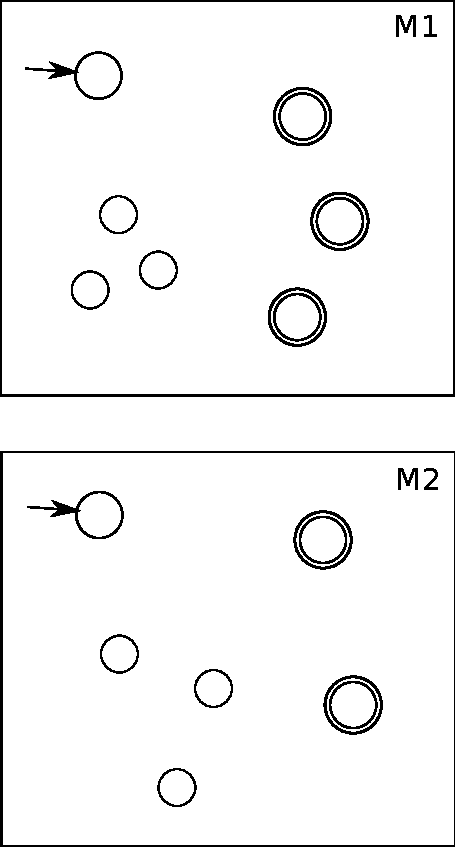
\includegraphics[scale=0.4]{images/union_before.pdf}
      \end{center}
    }
  
    \pause

    \column{.5\textwidth} {
      \begin{center}
        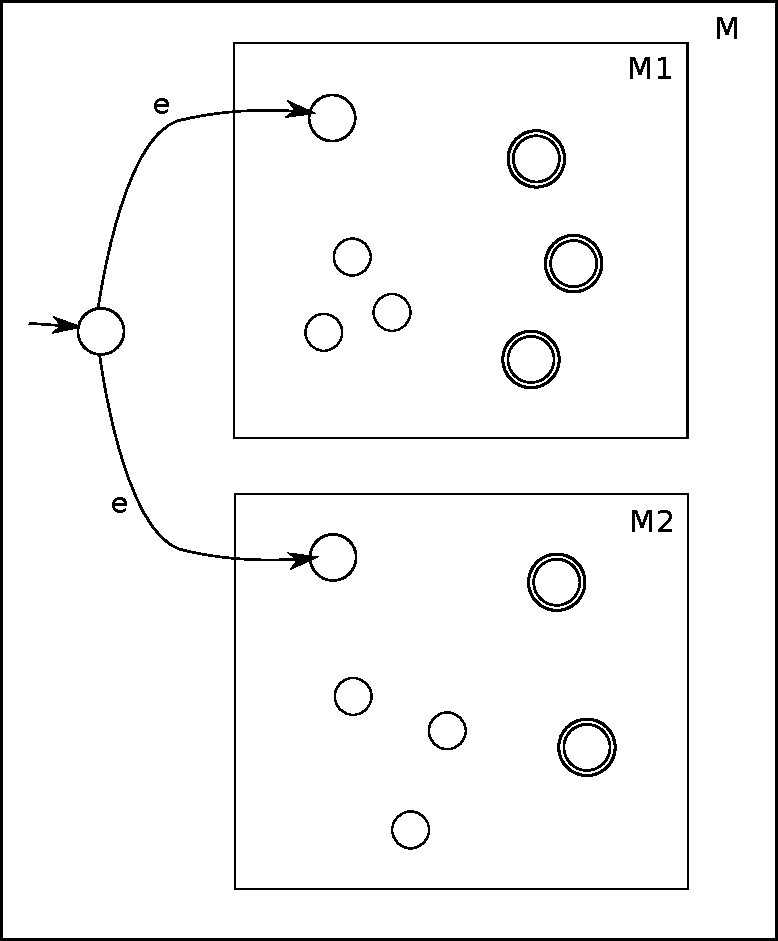
\includegraphics[scale=0.4]{images/union_after.pdf}
      \end{center}
    }
  
  \end{columns}
}

\frame{
  \frametitle{Concatenation: idea}

    \begin{center}

    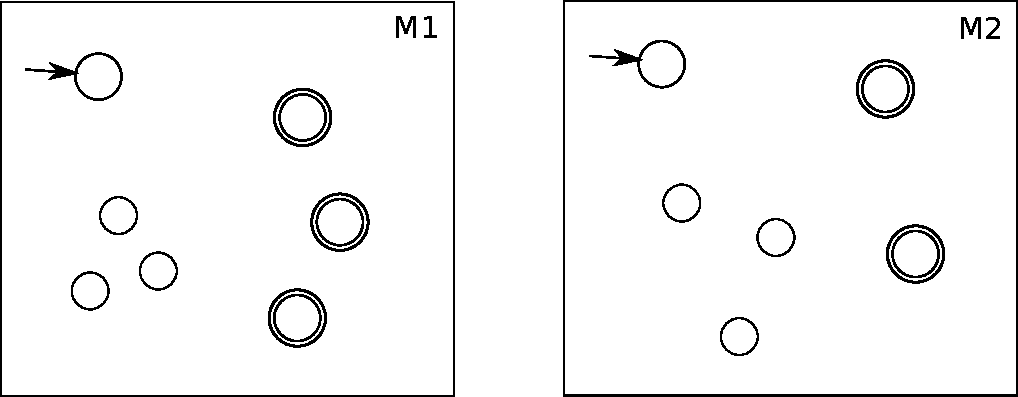
\includegraphics[scale=0.4]{images/concat_before.pdf}
  
    \vspace{0.2in}
    \pause

    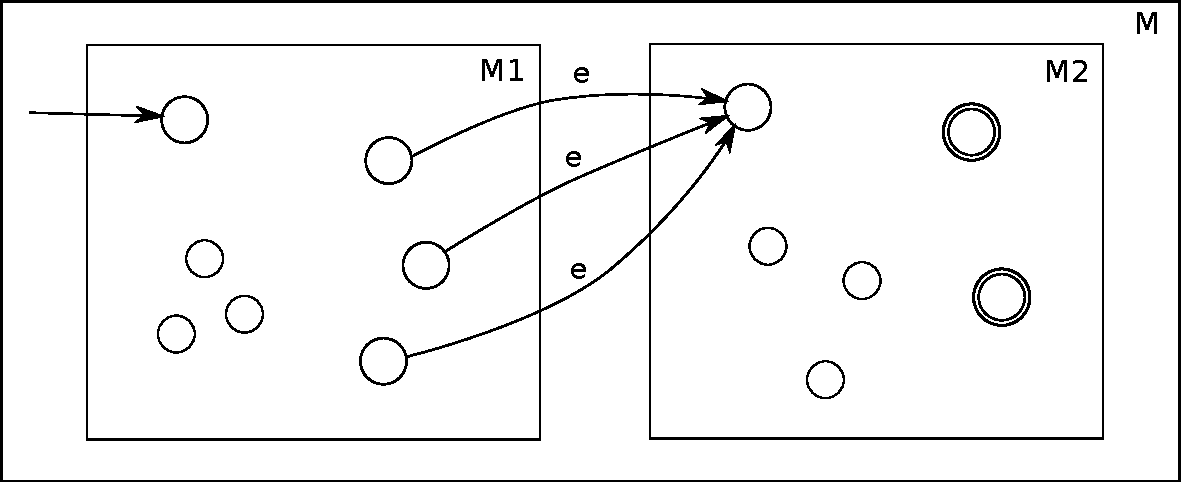
\includegraphics[scale=0.4]{images/concat_after.pdf}
  \end{center}
  
}

\frame{
  \frametitle{Stronger claim}

  Our goal is to prove:
  \begin{lemma}
    Every regular language is accepted by a nondeterministic
    finite-state automaton.
  \end{lemma}

  \pause

  But we will prove a ``stronger'' claim.
  
  \begin{lemma}[Thompson's algorithm]
    Every regular language is accepted by a nondeterministic
    finite-state automaton with {\color{red}\em exactly one accepting state,
      which is different from its start state}.
  \end{lemma}
}

\frame{

  \begin{proof}[Proof (Thompson's algorithm)]
    Consider any regular expression $R$ over alphaget $\Sigma$.  We
    prove that there is an NFA $N$ that accepts the language described
    by $R$ by induction.

    {\color{blue} {\bf Induction hypothesis:} for any subexpression
      $S$ of $R$, there is an NFA that accepts the language described
      by $S$.}

    We denote an NFA with this notation: \pause

    There are 6 cases: \pause
    \begin{itemize}
    \item $R=\emptyset$: \pause
    \item $R=\epsilon$: \pause
    \item $R=a$ for some $a\in\Sigma$: \pause
    \item $R=ST$ for some regular expression $S$ and $T$: \pause
    \item $R=S+T$ for some regular expression $S$ and $T$: \pause
    \item $R=S^*$ for some regular expression $S$: \pause
    \end{itemize}

    In all cases, the language $L(R)$ is accepted by an NFA with
    exactly one accepting state which is different from its start
    state, as required.
  \end{proof}

}


\frame{
  \frametitle{Example: $\cone+\czero\czero$}
}

\frame{
  \frametitle{Example: $(\cone+\czero\czero)^*$}
}

\frame{
  \frametitle{Example: $(\cone+\czero\czero)^*+\cone^*\czero$}
}

\frame{
  \frametitle{NFA to Regular expressions}

}

\frame{
  \frametitle{State elimination: example 1}

  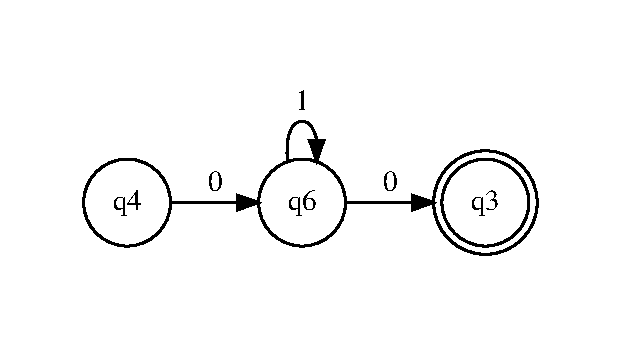
\includegraphics[width=2.5in]{images/m5-q6-before.pdf}

}

\frame{
  \frametitle{State elimination: example 2}

  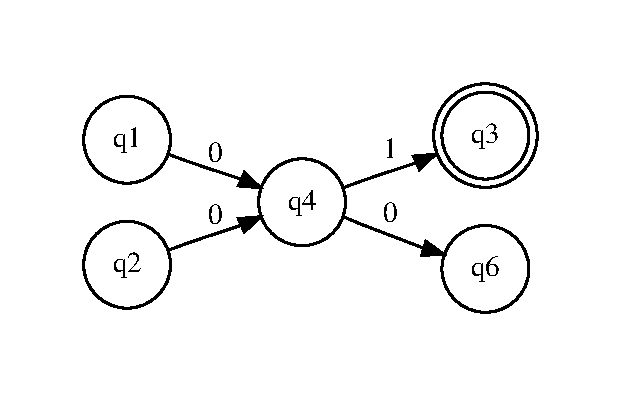
\includegraphics[width=2.5in]{images/m5-q4-before.pdf}

}

\frame{
  \frametitle{State elimination: example 3}

  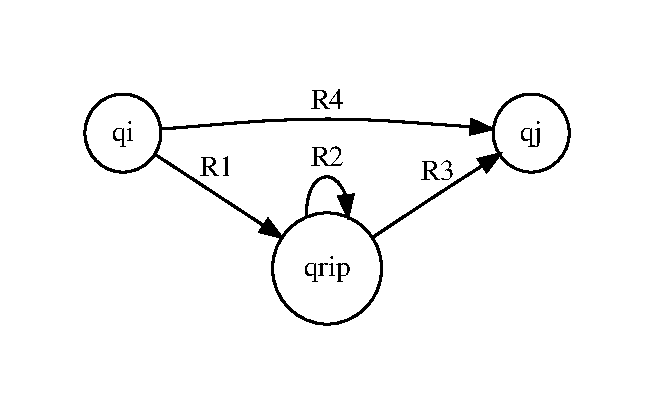
\includegraphics[width=2.5in]{images/rip1.pdf}

}
